\chapter{Probleembeschrijving}
\label{chap:Probleembeschrijving}
Dit hoofdstuk beschrijft het probleem van automatische afbeeldingsbeschrijving. Een eerste sectie gaat over het concrete vraagstuk en de situering binnen de computerwetenschappen. Een tweede sectie beschrijft de praktische toepassingen van een systeem dat in staat is om automatisch afbeeldingen te beschrijven. Een volgende sectie biedt toelichting bij de meest gebruikte datasets voor het trainen en evalueren van systemen die een oplossing bieden voor dit probleem. Tot slot geeft een laatste sectie een overzicht van de concrete onderzoeksvragen.

\section{Omschrijving en situering binnen computerwetenschappen}
\label{sec:Omschrijving en situering}
Voor een mens is het beschrijven van een afbeelding zeer eenvoudig. Hij ziet in een oogopslag welke objecten zich in de foto bevinden en in welke relaties ze zich verhouden. Het taalgevoel eigen aan de mens maakt het bedenken van een beschrijvende zin allesbehalve problematisch.
Voor een computer is dit vraagstuk echter veel complexer.

Automatische afbeeldingsbeschrijving bevindt zich op het snijpunt van computervisie (CV) en natuurlijke taalverwerking (NLP) door de combinatie van afbeeldingen en tekst. Klassiek gezien worden deze disciplines beschouwd als losstaande vakgebieden. Voor het beschrijven van afbeeldingen is er echter nood aan een combinatie van technieken uit beide vakgebieden. Het systeem moet als eerste in staat zijn de verschillende objecten in de foto te herkennen. De computer moet ook een notie hebben van wat elk object precies is en hoe de objecten zich verhouden. Daarna pas kan het systeem een grammaticaal correcte, vloeiende zin genereren. Om dit laatste te doen is het nodig dat de computer over enige vorm van ``taalgevoel'' kan beschikken. Een ander probleem is de ambigu\"iteit die onvermijdelijk optreedt bij het gebruik van taal en beeld: woorden kunnen verschillende betekenissen hebben, afbeeldingen hebben verschillende mogelijke beschrijvingen, \ldots

Het genereren van beschrijvingen is nauw gerelateerd aan andere, eerder onderzochte problemen. Het opzoeken van afbeeldingen is hiervan het bekendste voorbeeld. Op basis van een aantal sleutelwoorden, of een volledige zin, zoekt een algoritme in een database naar de afbeelding die het beste overeenkomt met de vraag. In grote lijnen is dit het omgekeerde van wat deze masterproef beoogt. Dit werk zet afbeeldingen om in tekstfragmenten, terwijl het opzoeken van afbeeldingen een tekstfragment omzet in een afbeelding.

Aan de NLP-kant zijn veel aspecten van de automatische afbeeldingsbeschrijving gelijkaardig aan de automatische machinevertaling. Hierbij probeert een systeem zinnen of volledige teksten automatisch te vertalen van een brontaal naar een doeltaal. Voor dit probleem bestaan verschillende types van systemen. Wanneer een systeem concreet de vertaling van een zin woord per woord maakt, werkt het dikwijls met een geleerd taalmodel. Dit taalmodel probeert het taalgevoel van de mens te simuleren. Naar analogie met machinevertaling beschouwt de literatuur afbeeldingsbeschrijving dikwijls als automatische vertaling van afbeeldingen naar het Engels.

Het automatisch herkennen van objecten in afbeeldingen vormt \'e\'en van de meest onderzochte vraagstukken in het domein van de computervisie. Zoals eerder gezegd, is er niet enkel nood aan algoritmes die vormen detecteren in afbeeldingen, maar moet er ook een adequate labeling van de gedetecteerde vormen zijn. Een zeer gelijkaardig probleem is het classificeren van een volledige afbeelding, waarbij de hele sc\`ene een label krijgt in plaats van de gedetecteerde objecten.

De concrete probleemstelling voor het vraagstuk van afbeeldingsbeschrijving is de volgende: \emph{``Genereer een vloeiende, grammaticaal correcte Engelse zin die beschrijft wat er op een nooit eerder geziene foto staat''}. Een voorbeeld van twee afbeeldingen met automatisch gegenereerde zinnen is te zien in figuur~\ref{fig:examplecaptions}.

\begin{figure}[tb]
	\centering
	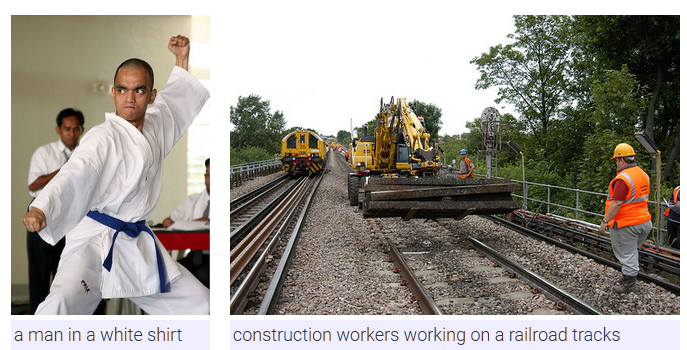
\includegraphics[width= 0.85\linewidth]{Images/caption.png}
	\caption{Twee afbeeldingen en hun gegenereerde beschrijving}
	\label{fig:examplecaptions}
\end{figure}

Meer specifiek legt dit proefschrift de focus op het ontwikkelen van een taalmodel dat beter presteert dan een aantal recente systemen. Deze recente systemen vertonen vaak dezelfde gebreken: de gegenereerde zinnen zijn korter dan de zinnen uit de trainingsverzameling en het aantal unieke woorden ligt vrij laag. Daarnaast zijn er verschillende beschrijvingen die kleine of grotere fouten vertonen in de overeenkomst met de ingevoerde afbeelding. Het is de bedoeling van deze masterproef om voor deze gebreken een oplossing te vinden. Dit gebeurt door het toevoegen van extra semantische informatie en het verbeteren van de zoekmethode om zinnen op te bouwen.


\section{Toepassingen}
Het oplossen van dit probleem heeft naast academische ook praktische toepassingen. Zo maakt een afbeeldingsbeschrijvend systeem het mogelijk om voor slechtzienden te beschrijven wat er op de afbeeldingen van een webpagina staat. Indien een browser voor slechtzienden bovendien in staat is om geschreven tekst uit te spreken, krijgen zij hierdoor betere toegang tot het internet. Ook internetgigant Facebook ziet het nut van zulke systemen. Daarom hebben hun ontwikkelaars tijdens het schrijven van deze masterproef een nieuwe functie toegevoegd aan Facebook, die in staat is afbeeldingen op hun website te beschrijven voor slechtzienden~\cite{facebook}.

Daarnaast zijn ook toepassingen denkbaar voor het automatisch ordenen van foto's op basis van dezelfde woorden in de gegenereerde beschrijvingen. Denk bijvoorbeeld concreet aan een filter die afbeeldingen filtert met het woord \texttt{sneeuw} in de beschrijving. 

Meer algemeen maakt het ook het zoeken naar afbeeldingen op het web eenvoudiger. Zo cre\"eert dergelijk systeem de mogelijkheid om naar sleutelwoorden of zinnen te zoeken in de automatisch gegenereerde beschrijvingen. Dit is directer dan zoeken op basis van de afbeeldingsnaam, tekst in de omgeving of tags van de afbeelding. Deze gegevens zijn vaak onvolledig, fout of nietszeggend, waar een automatisch gegenereerde beschrijving een oplossing biedt.

Een andere mogelijke oplossing is het integreren van een afbeeldingsbeschrijvend systeem in een zelfrijdende auto. Op basis van objecten die zich rond de auto bevinden, kan een systeem aangepaste meldingen opmaken voor de inzittenden en voor het rij-algoritme. Op die manier is er meer onderscheid dan het zwart-witte contrast tussen ``iets zien'' en ``niets zien''. Voor een plastieken zak hoeft de auto niet te stoppen, terwijl een dier op de rijbaan wel een reactie dient op te wekken.

\section{Datasets}
\label{sec:Datasets}
Deze sectie beschrijft de drie meest gebruikte datasets voor training en evaluatie van modellen voor afbeeldingsbeschrijving: Flickr8k, Flickr30k en MS COCO.

\subsection{Flickr8k}
\label{par:Flickr8k}
De Flickr8k dataset~\cite{Hodosh2013} bevat 8.092 foto's die focussen op mensen en dieren (vooral honden) die een actie uitvoeren. De foto's zijn manueel geselecteerd om de grootst mogelijke vari\"eteit te garanderen. De selectie gebeurde vanuit Flickr\footnote{\url{https://flickr.com}}, een online portaal voor het hosten van afbeeldingen.

Mensen met Engels als moedertaal stellen de bijhorende beschrijvingen manueel op. De onderzoekers maken gebruik van~\emph{Amazon Mechanical Turk workers}\footnote{\url{https://www.mturk.com}}, een online platform om ``Human Intelligence Tasks'' te laten uitvoeren door mensen. Voor een kleine vergoeding kan iedereen die dat wenst de taken oplossen. 

Een voorafgaande test van de personen die de zinnen schrijven moet de correctheid van de beschrijvingen garanderen. Op basis van een aantal eenvoudige richtlijnen moeten de proefpersonen beschrijvingen voor de afbeeldingen opstellen. De vraag is om objecten en acties te beschrijven in een simpele maar volledige zin met voldoende adjectieven. Er is geen harde restrictie op het aantal woorden in de beschrijvingen~\cite{Hockenmaier2014}.

Eenzelfde afbeelding kan tot verschillende beschrijvingen leiden: sommige mensen focussen op de actie, anderen leggen de nadruk op de persoon die de actie uitvoert, \ldots\  De zinnen \texttt{A man is skiing down a hill} en \texttt{A man is going down a hill on his skis} beschrijven dezelfde foto, maar doen dit op een verschillende manier. Om deze rijkdom in de taal te kunnen weergeven zijn er vijf zinnen per afbeelding opgenomen in de dataset.

De dataset is verdeeld in drie delen voor training, validatie en testen. De validatie- en testset bevatten elk 1.000 foto's, de trainingsset bevat de overige 6.092.


\subsection{Flickr30k}
\label{par:Flickr30k}
De Flickr30k dataset~\cite{Young2014} is een uitbreiding van Flickr8k. Deze uitbreiding is ontstaan vanuit \'e\'en van de basisprincipes in het machinaal leren: \emph{``Hoe groter de trainingsset, hoe beter het getrainde systeem kan zijn''}. In totaal zijn er 31.783 foto's, met elk 5 beschrijvingen. Het proces dat gebruikt is om de dataset op te stellen is hetzelfde als bij Flickr8k. Ook hier bestaan de test- en validatieset uit 1.000 foto's, met de resterende 29.783 afbeeldingen in de trainingsset.

\subsection{Flickr30k Entities}
\label{sec:entities}
De dataset Flickr30k Entities~\cite{Plummer2015} is gebaseerd op de Flickr30k dataset. Ze bevat een groot aantal annotaties en omspannende rechthoeken, alsook verbanden tussen beide. Deze verbanden kunnen een bron zijn van extra informatie.

De dataset is ontstaan op basis van een eenvoudig idee. De makers zien in dat een ``standaard'' afbeeldingsbeschrijvend systeem een globaal verband leert tussen een foto en een zin, zonder echt rekening te houden met de overeenkomsten tussen entiteiten op de foto en in de zin. Er zijn vrij recent wel een aantal systemen ontwikkeld die een projectie maken van afbeeldingsregio's naar beschrijvingen. Deze systemen veronderstellen echter dat deze verbanden latent zijn. Hier probeert de nieuwe Entities dataset verandering in te brengen, door de verbanden tussen beschrijving en foto te expliciteren.

De dataset is gebaseerd op de meer dan 30.000 afbeeldingen uit de Flickr30k dataset~\cite{Young2014} met de bijhorende beschrijvingen. De makers brengen een uitbreiding hiervan, met een set van bijna 250.000 \emph{coreference chains}, die verbanden aangeven tussen regio's uit de afbeeldingen en zinsdelen uit de beschrijvingen. Deze aanpak lijkt op wat de MS COCO~\cite{Lin2014} dataset biedt, maar de objecten in de COCO dataset zijn onafhankelijk van de beschrijvingen gedetecteerd. Figuur~\ref{fig:entities} toont een aantal voorbeelden van annotaties en referenties uit de Entities dataset, terwijl figuur~\ref{fig:cocoexamples} toont hoe de verschillende objecten in de COCO dataset worden opgeslagen. Het is duidelijk dat er bij de COCO dataset geen rechtstreeks verband is met de beschrijvingen. Dit verband is net wat Flickr30k Entities zo interessant maakt voor het extraheren van extra semantische informatie. Het netwerk leert dan niet enkel een relatie tussen een gegeven afbeelding en de uiteindelijke zin, maar ook het verband tussen de encodering van alle links die in de afbeelding zitten en de uiteindelijk gegenereerde zin.

\begin{figure}[!tb]
	\centering
	\begin{tabular}[t]{cc}
		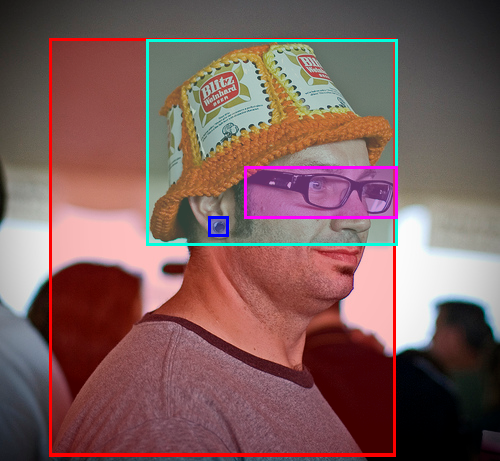
\includegraphics[height=3.0in]{Images/example_hat.png} \vspace{-3mm}&
		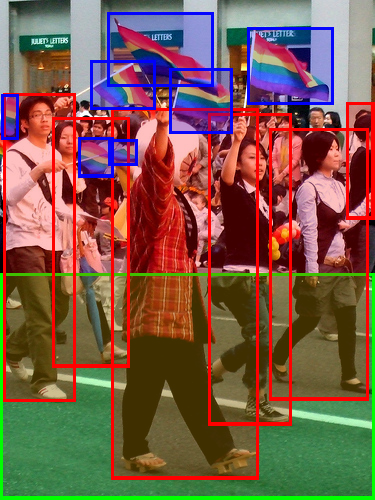
\includegraphics[height=3.0in]{Images/example_parade.png}\\
		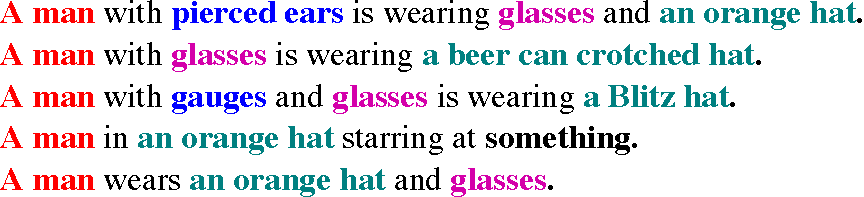
\includegraphics[valign = T,width=.4\columnwidth]{Images/example_hat_text.pdf}&
		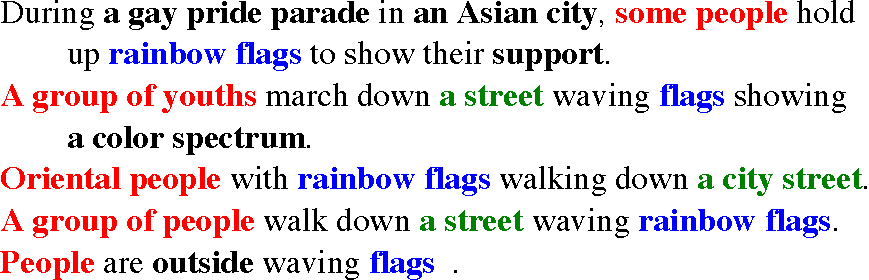
\includegraphics[valign = T,width=.4\columnwidth]{Images/example_parade_text.pdf}
		\end{tabular}
		\caption[Voorbeelden van Flickr30k Entities annotaties]{Voorbeelden van Flickr30k Entities annotaties. De kleur van de zinsdelen komt overeen met de kleur van de omspannende rechthoeken op de afbeelding~\cite{Plummer2015}.}
		\label{fig:entities}
		\end{figure}
		
		\begin{figure}
			\centering
			\subfloat{
				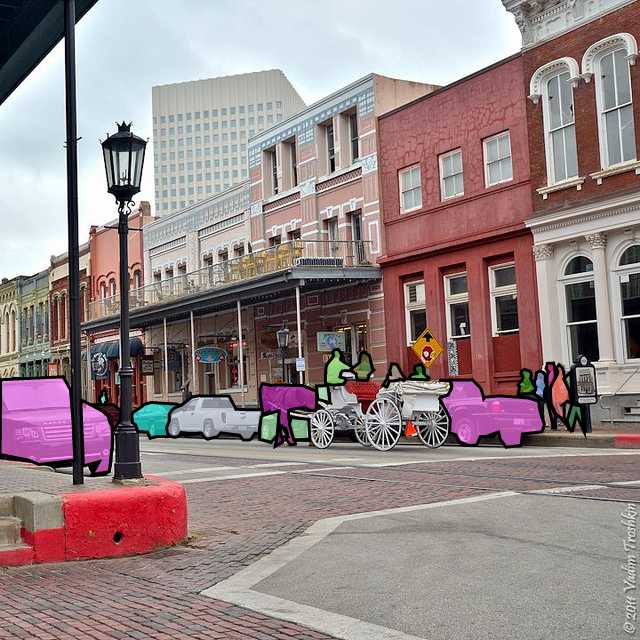
\includegraphics[width=0.47\linewidth]{Images/coco_example1.png}}\hfill
				\subfloat{
					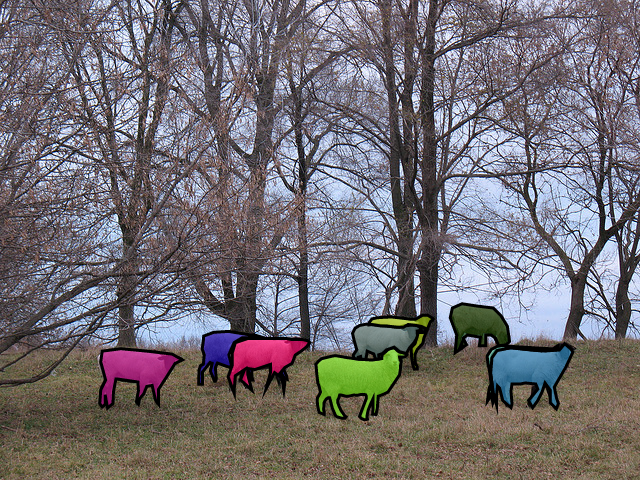
\includegraphics[width=0.47\linewidth]{Images/coco_example2.png}}
					\caption[Voorbeelden van geannoteerde afbeeldingen uit de \mbox{MS COCO dataset}]{Voorbeelden van geannoteerde afbeeldingen uit de \mbox{MS COCO dataset}. Elk gekleurd object behoort tot \'e\'en van de objectcategorie\"en gedefinieerd door de makers~\cite{Lin2014}.}
					\label{fig:cocoexamples}
					\end{figure}


\subsection{MS COCO}
\label{par:MS COCO}
De Microsoft Common Objects in COntext dataset (MS COCO)~\cite{Lin2014} staat los van de Flickr datasets en probeert een ander type van afbeelding te brengen. Ze bevat meer dan 330.000 afbeeldingen die elk vijf beschrijvingen hebben. 

MS COCO probeert meer te bieden dan ``standaard'' foto's. De auteurs maken een onderscheid tussen afbeeldingen van iconische objecten en iconische sc\`enes, en niet-iconische afbeeldingen. Iconische afbeeldingen vormen typisch de eerste zoekresultaten bij een Google Image Search, maar ze bevatten te weinig informatie. Iconische objectafbeeldingen bevatten een centraal geplaatst object. Iconische sc\`eneafbeeldingen bevatten een sc\`ene, meestal zonder aanwezigheid van mensen, vanuit een canonisch aanzicht. Bij canonische aanzichten staat de camera quasi loodrecht op de gefotografeerde sc\`ene, zij het in boven-, onder-, voor- of zijaanzicht. Hoewel iconische afbeeldingen kunnen leiden tot zeer goede objectdetecties, is er weinig tot geen contextuele informatie aanwezig. Hierdoor zijn beschrijvingen van dit type afbeelding minder interessant.  Niet-iconische afbeeldingen brengen algemeen gezien een compositie van verschillende objecten en personen, gefotografeerd vanuit een niet-canonische hoek. Figuur~\ref{fig:cocotypes} toont duidelijk het verschil tussen iconische en niet-iconische afbeeldingen.

\begin{figure}[tb]
	\centering
	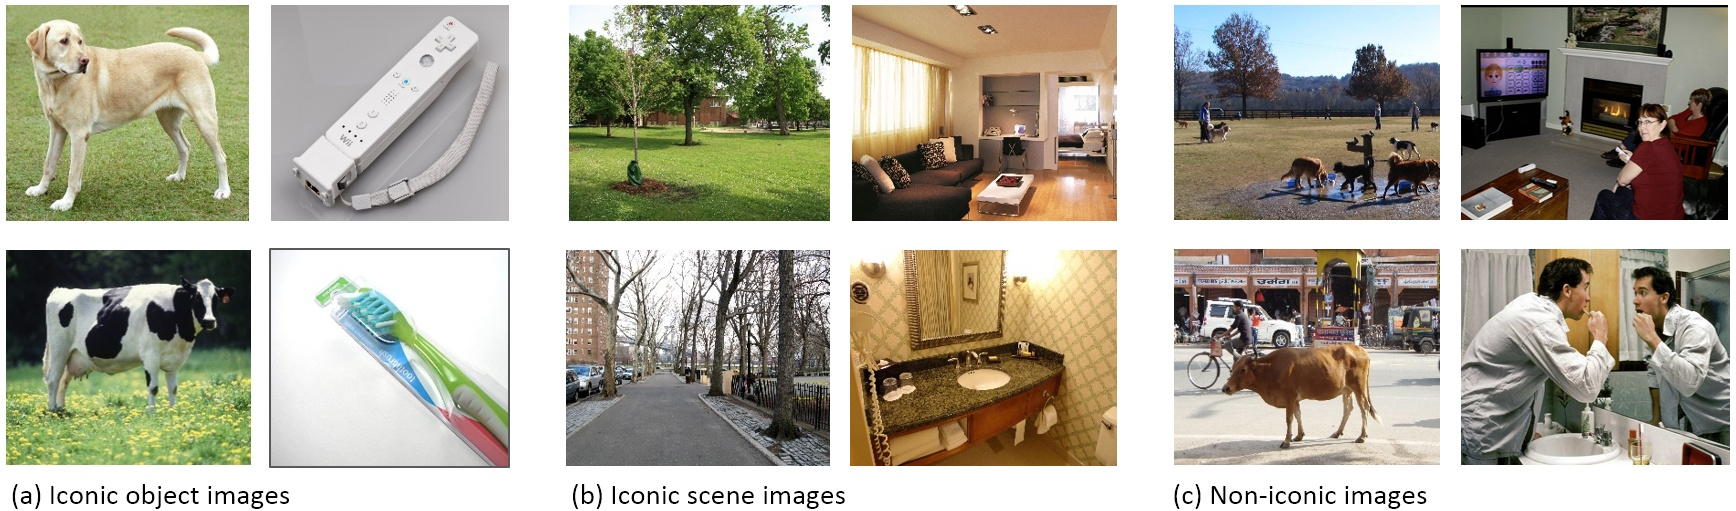
\includegraphics[width=\linewidth]{Images/iconic.jpg}
	\caption[Verschil tussen iconische en niet-iconische afbeeldingen]{Verschil tussen iconische en niet-iconische afbeeldingen~\cite{Lin2014}}
	\label{fig:cocotypes}
\end{figure}

Een ander belangrijk deel van de COCO-dataset zijn annotaties. Oudere datasets leggen de focus op classificatie, omgevende rechthoeken en segmentatie, terwijl \mbox{MS COCO} probeert om elk belangrijk object op de foto te annoteren. De afbeeldingen zijn gebaseerd op een lijst van objectcategorie\"en en zijn specifiek geselecteerd om niet-iconische sc\`enes te bevatten. De Flickr-datasets focussen niet expliciet op niet-iconische afbeeldingen en bevatten bijgevolg meer variatie in het type afbeeldingen.

Het genereren van de beschrijvingen bij de foto's gebeurt met \texttt{Amazon Mechanical Turk workers}, net zoals bij de Flickr-datasets. Uitgebreide instructies voor de workers garanderen dat elk belangrijk deel van de afbeelding voorkomt in de beschrijving~\cite{Rampf2015}. Figuur~\ref{fig:coco_ui} toont op welke wijze de proefpersonen een beschrijving moeten ingeven.

\begin{figure}[tb]
	\centering
	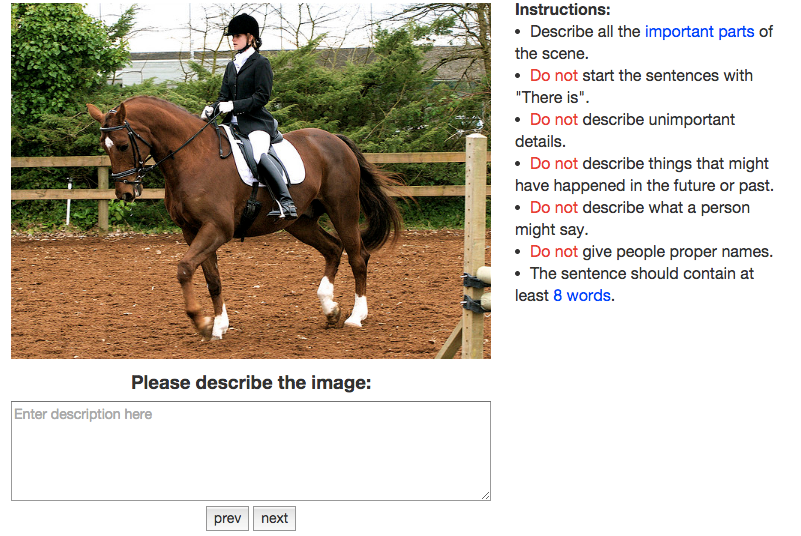
\includegraphics[width=0.8\linewidth]{Images/coco_UI.png}
	\caption[User interface voor het ingeven van afbeeldingsbeschrijvingen \mbox{MS COCO}]{User interface voor het ingeven van afbeeldingsbeschrijvingen \mbox{MS COCO}~\cite{Rampf2015}}
	\label{fig:coco_ui}
\end{figure}
\subsection{Gekozen dataset}
Dit werk gebruikt Flickr30k als dataset voor de training en evaluatie. Hoewel \mbox{MS COCO} groter is en meer complexe afbeeldingen bevat, maakt de grootte van Flickr30k snellere training van het systeem mogelijk. Daarnaast is deze dataset ook de meest gebruikte in de literatuur wat de vergelijking met bestaande systemen mogelijk maakt. 

\section{Onderzoeksvragen}
Deze sectie bevat een overzicht van de concrete onderzoeksvragen van deze masterproef.
\begin{enumerate}
	\item Welke vormen van semantische informatie kunnen op een haalbare manier verbetering bieden voor bestaande systemen? 
	\item Hoe kan semantische informatie worden toegevoegd aan de twee bestudeerde systemen?
	\item Wat is de invloed van het aanpassen van systeemspecifieke parameters? 
	\item Hoe presteren verschillende types van semantische informatie ten opzichte van elkaar? 
	\item Welke invloed ondervinden de beschouwde types semantische informatie van trainingsdata die ruis bevat?
	\item Hoe kunnen we langere, minder algemene zinnen genereren? 
\end{enumerate}

\section{Besluit}
Deze masterproef focust op het verbeteren van een bestaand systeem dat in staat is om afbeeldingen te beschrijven. Deze beschrijvingen moeten grammaticaal correcte, vloeiende Engelstalige zinnen zijn. Dit probleem bevindt zich op het snijpunt van CV en NLP en is nauw verbonden met andere problemen binnen deze domeinen. Naast het academisch nut van het oplossen van dit complexe probleem heeft de oplossing ook praktische toepassingen. Zo dient het al in toepassingen die slechtzienden helpen met het bekijken van afbeeldingen op het internet. Om dit probleem op te lossen zijn er drie frequent gebruikte datasets waarvan \mbox{MS COCO} de grootste en wellicht beste is. Flickr30k vormt een uitbreiding op Flickr8k en bevat minder en eenvoudigere afbeeldingen dan MS COCO. Omwille van de kleinere grootte en het frequentere gebruik in de literatuur traint en evalueert het systeem van deze masterproef met Flickr30k. 

Het volgende hoofdstuk biedt een overzicht van gebruikte methodes en modellen uit de literatuur om het hiervoor geschetste probleem op te lossen.
%%% Local Variables: 
%%% mode: latex
%%% TeX-master: "masterproef"
%%% End: 